\documentclass[11pt,a4paper]{article}
\usepackage[margin=1in]{geometry}
\usepackage{graphicx}
\usepackage{booktabs}
\usepackage{amsmath,amssymb}
\usepackage{multirow}
\usepackage{hyperref}
\usepackage{xcolor}
\usepackage{float}
\usepackage{caption}
\usepackage{subcaption}

\definecolor{healthy}{RGB}{46,139,87}
\definecolor{warning}{RGB}{204,153,0}
\definecolor{danger}{RGB}{178,34,34}

\title{Experiment Report: \texttt{spec27\_d512\_4b\_k2} (130K)\\[0.3em]
\large Extended Proxy Tape Training --- L1 Eta Collapse Under Prolonged Proxy Gradients}
\author{NL\_Hecate Research}
\date{March 17, 2026}

\begin{document}
\maketitle

\begin{abstract}
This report documents the \texttt{spec27\_d512\_4b\_k2} extended experiment: a 130K-step run
(30K initial + 100K warm restart) using Spec~27's per-level tape strategy (L0=exact, L1=proxy)
on the standard d=512, 4-block, k=2 CMS configuration. The run extends the previously validated
30K proxy experiment to test long-horizon proxy training.

The headline finding is \textbf{L1 eta collapse}: after step $\sim$57K, Block~0's L1 output gate
drops from $\sim$0.95 to oscillating 0.15--0.75 (mean $\sim$0.45--0.55), while L0 eta saturates
to 1.0. The model is progressively suppressing L1's output contribution under prolonged proxy training.
Despite this, loss continues to improve (smoothed 3.94 at 30K $\to$ 2.60 at 129K), meaning the model
adapts by routing information through L0.

Key results:
\begin{itemize}
    \item \textbf{Loss}: 11.0 $\to$ 2.72 (phase 1, 30K), warm restart $\to$ 2.60 (phase 2, 129K).
    \item \textbf{L1 eta collapse}: Block~0 L1 eta drops from 0.96 to $\sim$0.48 after step 57K.
    \item \textbf{L1 alpha floor-pinning}: L1 alpha hits the 0.80 floor in Blocks 0/1/2 by step 60K.
    \item \textbf{Block 2 L1 theta}: Continues rising from 0.45 (30K) to 0.88 (125K) --- the sole block where proxy L1 actively learns.
    \item \textbf{Block CV collapse}: Depth specialization drops from 0.55 to 0.18 --- blocks homogenize.
    \item \textbf{Throughput}: 1,186 tok/s mean, consistent across both phases.
    \item \textbf{18 gradient spikes}, including a 36.6-norm event at step 117,584.
\end{itemize}
\end{abstract}

\tableofcontents
\newpage

%=============================================================================
\section{Experiment Configuration}
%=============================================================================

\begin{table}[H]
\centering
\caption{Run configuration. Warm restart at step 30K with fresh 100K cosine schedule.}
\begin{tabular}{ll}
\toprule
\textbf{Parameter} & \textbf{Value} \\
\midrule
\multicolumn{2}{l}{\textit{Architecture}} \\
\quad d\_model & 512 \\
\quad num\_heads & 8 \\
\quad n\_blocks & 4 \\
\quad params & 55,141,386 \\
\quad k / chunk\_sizes & 2 / [1, 8] \\
\quad composition & MAG \\
\quad memory\_rule & Titans LMM \\
\midrule
\multicolumn{2}{l}{\textit{Tape Strategy (Spec 27)}} \\
\quad tape\_strategies & [exact, proxy] \\
\quad tape\_multiplier & 1 \\
\quad tape\_device & GPU \\
\midrule
\multicolumn{2}{l}{\textit{Training --- Phase 1 (steps 0--30K)}} \\
\quad steps & 30,000 \\
\quad lr / warmup & 3e-4 / 500 \\
\quad optimizer & AdamW (GPU stacked) \\
\quad alpha\_floor & [0.8, 0.8] \\
\quad seed & 42 \\
\quad data & Dolmino-100B \\
\midrule
\multicolumn{2}{l}{\textit{Training --- Phase 2 (warm restart, steps 30K--130K)}} \\
\quad steps & 100,000 \\
\quad lr / warmup & 3e-4 / 500 (fresh cosine schedule) \\
\quad checkpoint & Phase 1 final (step 30K) \\
\bottomrule
\end{tabular}
\end{table}

\subsection{Two-Phase Structure}

The run consists of two build phases logged in the metrics:
\begin{enumerate}
    \item \textbf{Phase 1} (0--30K): Initial training from scratch. Cosine schedule over 30K steps.
          Final loss: 2.715, throughput: 1,182 tok/s, wall time: 3.61h.
    \item \textbf{Phase 2} (30K--130K): Warm restart from the phase 1 checkpoint with a fresh
          100K-step cosine schedule. The LR resets to 3e-4, causing a temporary loss spike at step 30K
          (smoothed loss jumps from $\sim$3.0 to $\sim$3.9) before the model re-adapts.
\end{enumerate}

\noindent The warm restart is visible in every metric as a discontinuity at step 30K: loss spikes,
gradient norms spike, and gate values shift. All analysis in this report accounts for this
phase boundary.

%=============================================================================
\section{Loss Trajectory}
%=============================================================================

\begin{figure}[H]
\centering

\includegraphics[width=\textwidth]{loss_ppl.pdf}
\caption{Full 130K loss and perplexity. The phase boundary at 30K is marked by a red dashed line.
Loss spikes at 30K due to the warm restart LR reset, then resumes descent. Final smoothed loss: 2.60.}
\end{figure}

\begin{table}[H]
\centering
\caption{Loss progression at key milestones (last-50 smoothed averages).}
\begin{tabular}{rrl}
\toprule
\textbf{Step} & \textbf{Smoothed Loss} & \textbf{Phase} \\
\midrule
1,000  & 4.88 & Phase 1 (early) \\
5,000  & 4.23 & Phase 1 (warmup complete) \\
10,000 & 3.91 & Phase 1 (mid) \\
20,000 & 3.41 & Phase 1 (late) \\
30,000 & 3.94 & Phase boundary (LR spike) \\
50,000 & 3.63 & Phase 2 (re-adapting) \\
75,000 & 2.73 & Phase 2 (converging) \\
100,000 & 2.82 & Phase 2 (plateau/oscillation) \\
125,000 & 2.77 & Phase 2 (late) \\
129,000 & 2.60 & Phase 2 (final) \\
\bottomrule
\end{tabular}
\end{table}

\noindent Notable features:
\begin{itemize}
    \item The loss at step 100K (2.82) is \textit{worse} than step 75K (2.73), suggesting the cosine
          schedule's declining LR creates a temporary plateau before the final descent.
    \item Phase 2 achieves a lower final loss (2.60) than phase 1 (2.72) despite the warm restart disruption.
    \item The model recovers from the LR spike in $\sim$20K steps (by step 50K), then improves further.
\end{itemize}

\subsection{Comparison with spec25 (First 30K)}

\begin{figure}[H]
\centering

\includegraphics[width=\textwidth]{comparative_loss.pdf}
\caption{Left: First 30K overlay comparing spec25 (all exact) with this run's first phase. Right: the full 130K trajectory.}
\end{figure}

\noindent The first 30K of this run replicates the spec25 result: loss curves are virtually
indistinguishable, confirming the 30K proxy validation holds even when the run continues beyond.

%=============================================================================
\section{Gradient Analysis}
%=============================================================================

\begin{figure}[H]
\centering

\includegraphics[width=\textwidth]{grad_norms.pdf}
\caption{Global gradient norm and block CV over 130K steps. The phase boundary produces a gradient
norm spike. Block CV drops from 0.55 to 0.18 --- depth specialization decreases over time.}
\end{figure}

\begin{figure}[H]
\centering

\includegraphics[width=0.85\textwidth]{block_grad_norms.pdf}
\caption{Per-block gradient norms. The blocks converge toward each other during phase 2, consistent with the falling CV.}
\end{figure}

\begin{figure}[H]
\centering

\includegraphics[width=0.85\textwidth]{l0_grad_norms.pdf}
\caption{L0 per-block gradient norms. Block 0 continues to carry the strongest L0 gradient signal.}
\end{figure}

\subsection{Depth Specialization Collapse}

\begin{figure}[H]
\centering
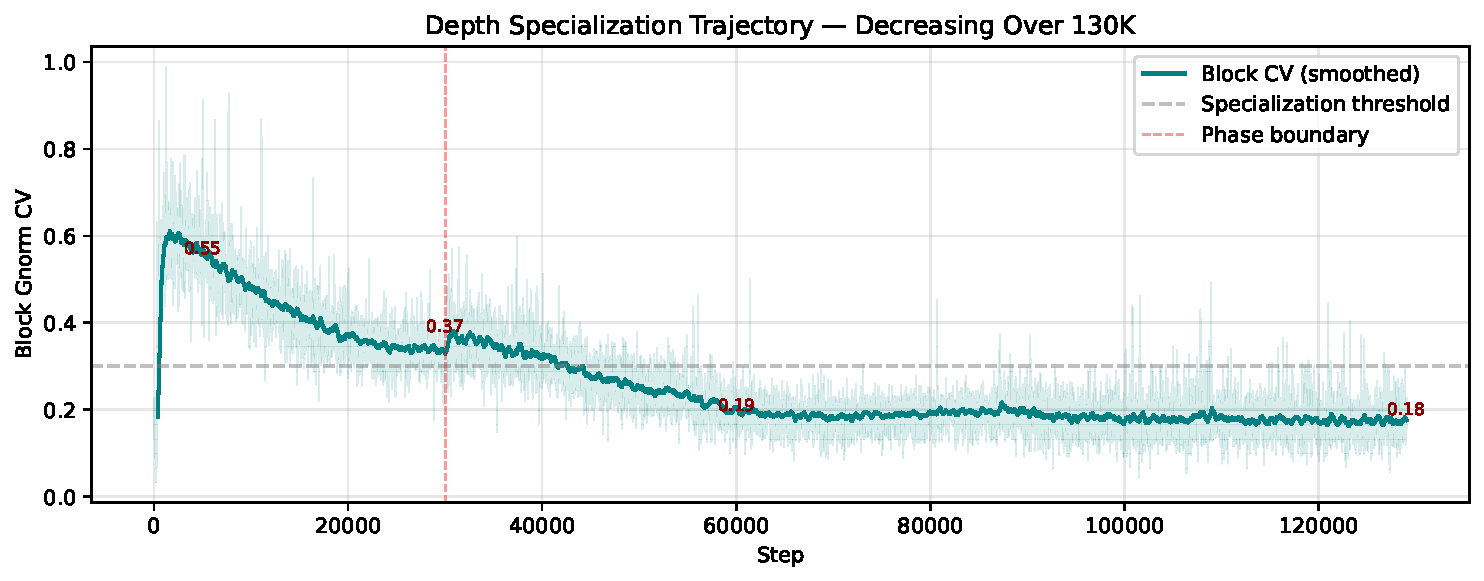
\includegraphics[width=0.85\textwidth]{block_cv_trajectory.pdf}
\caption{Block gnorm CV trajectory with annotated values. The CV drops below the 0.3 specialization
threshold by step $\sim$45K and continues declining to 0.18 at step 129K.}
\end{figure}

\begin{table}[H]
\centering
\caption{Block CV at milestones.}
\begin{tabular}{rl}
\toprule
\textbf{Step} & \textbf{Block CV} \\
\midrule
5,000 & 0.549 \\
30,000 & 0.368 \\
60,000 & 0.188 \\
100,000 & 0.181 \\
129,000 & 0.176 \\
\bottomrule
\end{tabular}
\end{table}

\noindent The CV drops from 0.55 (phase 1 early, strong specialization) to 0.18 (phase 2 late, minimal
specialization). This is a qualitative shift: at d=512 k=2, extended training causes blocks to
\textbf{homogenize} their gradient norms. This contrasts with d=1024 (shakedown report), where CV
reached 0.84--0.92. Depth specialization appears to be model-size--dependent.

\subsection{Gradient Spikes}

\begin{table}[H]
\centering
\caption{All 18 gradient spikes ($>$10). Phase 2 has more spikes, including a 36.6-norm event.}
\small
\begin{tabular}{rrl}
\toprule
\textbf{Step} & \textbf{Grad Norm} & \textbf{Phase} \\
\midrule
0      & 13.86 & Init \\
10,784 & 15.05 & Phase 1 \\
13,072 & 12.17 & Phase 1 \\
15,800 & 15.41 & Phase 1 \\
23,672 & 11.80 & Phase 1 \\
27,576 & 12.51 & Phase 1 \\
\midrule
33,968 & 10.55 & Phase 2 (early) \\
35,816 & 11.10 & Phase 2 \\
45,384 & 11.83 & Phase 2 \\
50,640 & 12.01 & Phase 2 \\
96,936 & 13.12 & Phase 2 \\
101,296 & 13.89 & Phase 2 \\
115,720 & 19.34 & Phase 2 (late) \\
117,360 & 15.54 & Phase 2 \\
\textbf{117,584} & \textbf{36.62} & \textbf{Phase 2 (max)} \\
123,208 & 14.45 & Phase 2 \\
124,944 & 13.60 & Phase 2 \\
128,536 & 11.43 & Phase 2 \\
\bottomrule
\end{tabular}
\end{table}

\noindent Phase 1 had 6 spikes (consistent with the 30K-only report). Phase 2 adds 12 more, with the
late-training cluster (steps 115K--128K) containing the largest spike (36.6 at step 117,584). The model
does not diverge after any spike --- gradient clipping (max\_grad\_norm=1.0) contains all of them.

%=============================================================================
\section{Gate Diagnostics: The Headline Finding}
%=============================================================================

This section documents the three correlated phenomena that define the extended proxy training signature:
L1 eta collapse, L1 alpha floor-pinning, and L0 eta saturation.

\subsection{L1 Eta Collapse (The Headline)}

\begin{figure}[H]
\centering
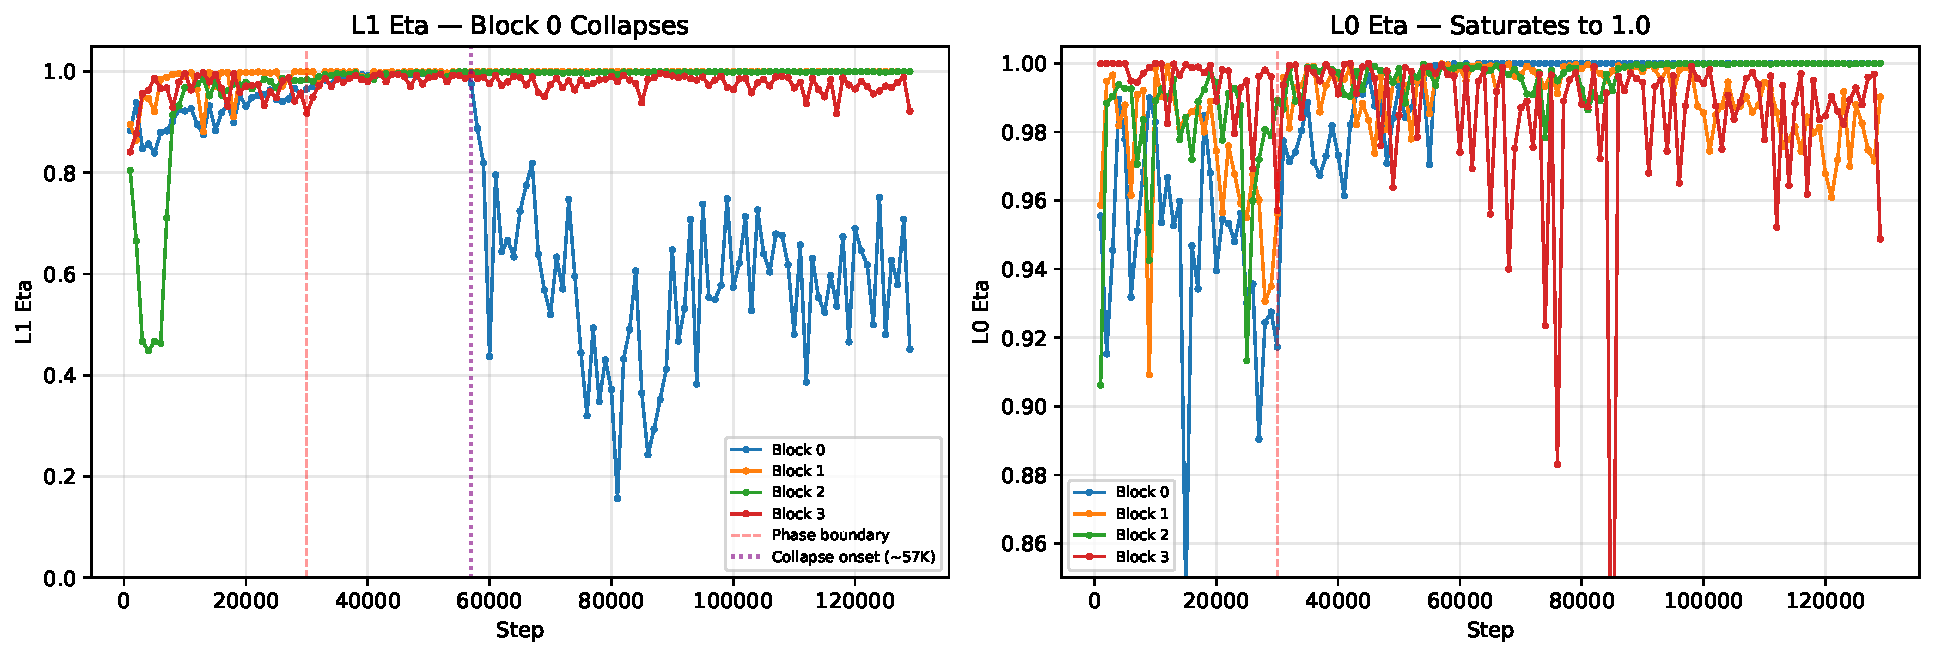
\includegraphics[width=\textwidth]{eta_collapse.pdf}
\caption{\textbf{The headline finding.} Left: Block~0's L1 eta drops from $\sim$0.96 to oscillating
0.15--0.75 after step $\sim$57K. Other blocks' L1 eta remains near 1.0. Right: L0 eta saturates
to 1.0 across all blocks by step 57K.}
\end{figure}

\begin{table}[H]
\centering
\caption{Block 0 L1 eta at key milestones.}
\begin{tabular}{rl}
\toprule
\textbf{Step} & \textbf{B0 L1 Eta} \\
\midrule
1,000  & 0.883 \\
10,000 & 0.922 \\
29,000 & 0.955 \\
50,000 & 0.996 \\
75,000 & \textcolor{danger}{0.445} \\
100,000 & \textcolor{danger}{0.574} \\
125,000 & \textcolor{danger}{0.480} \\
\bottomrule
\end{tabular}
\end{table}

\noindent \textbf{Interpretation}: Under proxy gradients, L1's inner-loop learning rate (theta) stays
near zero (Blocks 0/1/3), so L1's memory barely updates. Over 130K steps, the outer-loop optimizer
learns that L1's output contribution is not worth routing through --- it suppresses the output gate.
Block~0 is most affected because it is the first block and receives the strongest gradient signal
for gate adjustment.

This is \textbf{not} a training failure --- loss continues to improve. It is an adaptive response:
the model routes information through L0 (which has exact gradients and theta=1.0) and progressively
shuts down L1's contribution in Block~0. Blocks 1--3 maintain high L1 eta ($>$0.95) because their
L1 signal, while also proxy-derived, is less redundant with their L0.

\subsection{L1 Alpha Floor-Pinning}

\begin{figure}[H]
\centering

\includegraphics[width=\textwidth]{alpha_pinning.pdf}
\caption{L1 alpha across all blocks. Blocks 0, 1, and 2 reach the alpha\_floor (0.80) by step 60K.
Block 3 oscillates between 0.83 and 0.96.}
\end{figure}

\noindent L1 alpha (retention) decreasing to the floor means the model wants L1 to \textbf{forget faster}.
Combined with low L1 theta (slow learning), this produces an L1 that barely writes new information
and rapidly forgets what it has. The floor constraint (0.80) prevents complete L1 memory erasure.

\subsection{L0 Eta Saturation}

L0 eta saturates to 1.0 in all blocks by step $\sim$57K (see Figure~5, right panel). This is the
complementary signal to L1 eta collapse: as L1's output gate closes, L0's opens fully. The model
commits entirely to L0 for output contribution, confirming L0 as the dominant level under proxy training.

\subsection{Full Gate Evolution}

\begin{figure}[H]
\centering

\includegraphics[width=\textwidth]{theta_evolution.pdf}
\caption{Theta evolution over 130K steps. L0 theta saturates to 1.0 (all blocks). L1 theta stays
near zero (Blocks 0/1/3) except Block~2, which rises to 0.88.}
\end{figure}

\begin{figure}[H]
\centering

\includegraphics[width=\textwidth]{alpha_evolution.pdf}
\caption{Alpha evolution. L0 alpha is mixed (Block~0 rises to 0.94, others near floor). L1 alpha
trends toward the 0.80 floor in all blocks.}
\end{figure}

\begin{figure}[H]
\centering

\includegraphics[width=\textwidth]{eta_evolution.pdf}
\caption{Eta evolution. Note the eta y-axis starts at 0.0 to show the full collapse range.}
\end{figure}

\subsection{Block 2 L1 Theta: The Persistent Anomaly}

\begin{figure}[H]
\centering
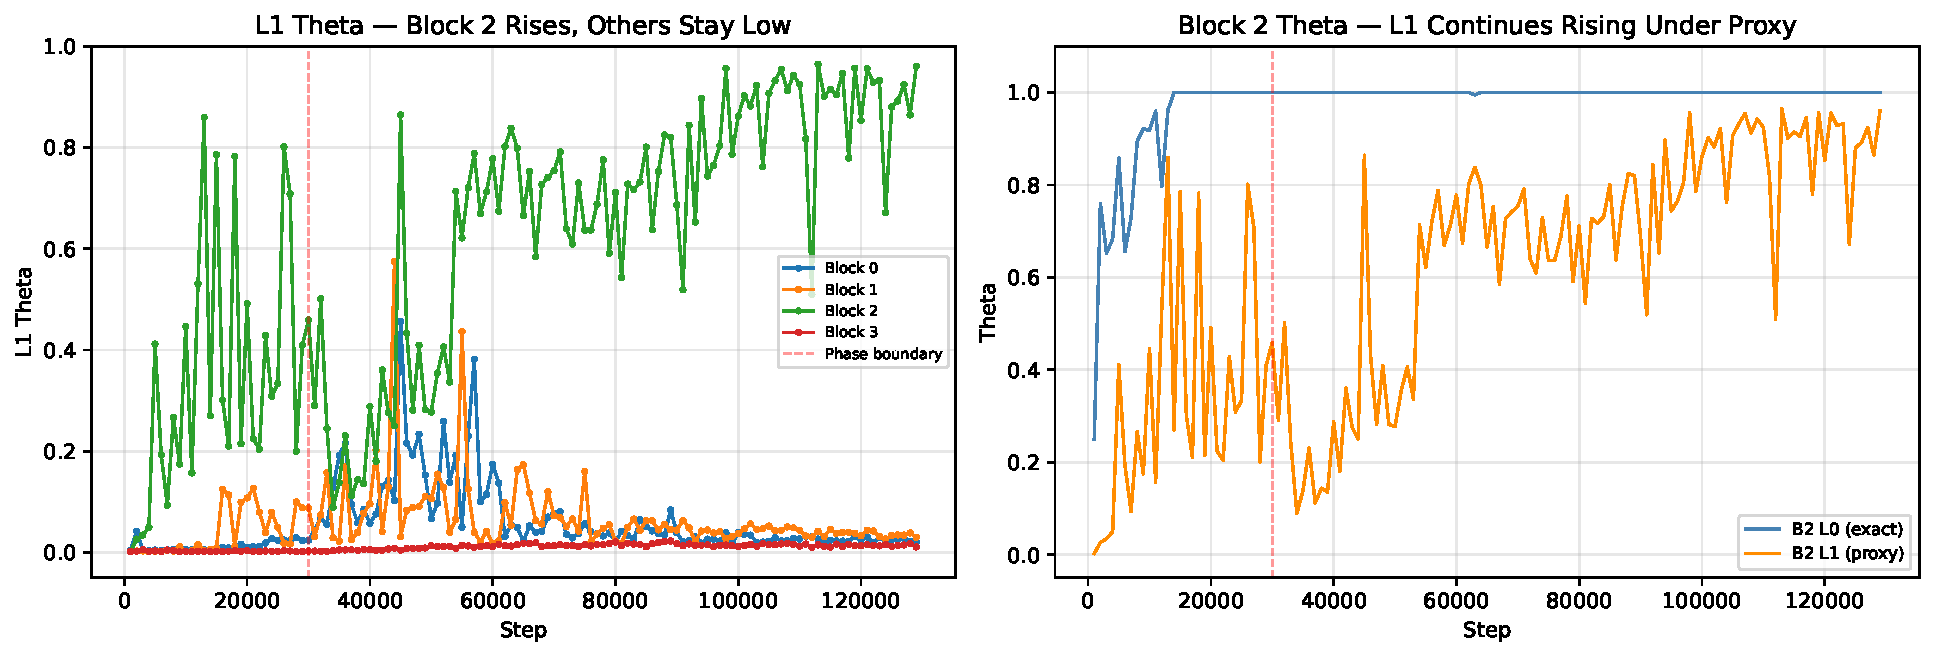
\includegraphics[width=\textwidth]{theta_block2.pdf}
\caption{Left: L1 theta across blocks --- Block~2 diverges dramatically from the others. Right:
Block~2's L1 theta continues rising from 0.45 (30K) to 0.88 (125K) under proxy gradients, while
L0 theta saturates to 1.0.}
\end{figure}

\noindent Block~2 is the only block where L1 proxy theta increases beyond 0.5. This anomaly appeared
in the 30K-only spec27 report ($\theta = 0.41$), and it \textbf{intensifies} under extended training
($\theta = 0.88$). The same block was anomalous at d=1024 in the shakedown ($\theta = 0.51$).
This suggests a depth-specific property of Block~2's position in the 4-block architecture: it
receives sufficient gradient signal through the output path alone to drive L1 learning, even
without the M trajectory chain that proxy truncates.

%=============================================================================
\section{Detailed Gate Comparison Table}
%=============================================================================

\begin{table}[H]
\centering
\caption{Gate values at four milestones across the 130K run.}
\small
\begin{tabular}{l|rrr|rrr|rrr|rrr}
\toprule
& \multicolumn{3}{c|}{Step 1K} & \multicolumn{3}{c|}{Step 29K} & \multicolumn{3}{c|}{Step 75K} & \multicolumn{3}{c}{Step 125K} \\
\textbf{B.L} & $\alpha$ & $\theta$ & $\eta$ & $\alpha$ & $\theta$ & $\eta$ & $\alpha$ & $\theta$ & $\eta$ & $\alpha$ & $\theta$ & $\eta$ \\
\midrule
B0L0 & .81 & .86 & .96 & .89 & 1.0 & .93 & .89 & 1.0 & 1.0 & .94 & 1.0 & 1.0 \\
B0L1 & .99 & .00 & .88 & .88 & .02 & .96 & .80 & .06 & \textcolor{danger}{.44} & .80 & .03 & \textcolor{danger}{.48} \\
B1L0 & .80 & .27 & .96 & .80 & 1.0 & .94 & .80 & 1.0 & 1.0 & .80 & 1.0 & .99 \\
B1L1 & .98 & .00 & .90 & .80 & .09 & 1.0 & .80 & .16 & 1.0 & .80 & .03 & 1.0 \\
B2L0 & .91 & .25 & .91 & .83 & 1.0 & .98 & .80 & 1.0 & 1.0 & .80 & 1.0 & 1.0 \\
B2L1 & .98 & .00 & .80 & .94 & .41 & .98 & .80 & .64 & 1.0 & .81 & \textcolor{warning}{.88} & 1.0 \\
B3L0 & .80 & .93 & 1.0 & .80 & .95 & 1.0 & .80 & 1.0 & 1.0 & .80 & 1.0 & .99 \\
B3L1 & .98 & .00 & .84 & .87 & .00 & .96 & .83 & .02 & .98 & .90 & .01 & .97 \\
\bottomrule
\end{tabular}
\end{table}

\noindent Reading the table column by column reveals the 130K trajectory:
\begin{itemize}
    \item \textbf{Step 1K}: L1 alpha high (0.98--0.99), L1 theta near zero, L1 eta moderate. L1 is retaining initialization and not learning.
    \item \textbf{Step 29K}: L1 alpha drops to 0.80--0.94 (approaching floor). Block~2 L1 theta reaches 0.41. Other L1 theta still near zero.
    \item \textbf{Step 75K}: L1 alpha at floor in Blocks 0--2. Block~2 L1 theta reaches 0.64. \textbf{Block~0 L1 eta collapses to 0.44.} L0 eta saturates to 1.0 in all blocks.
    \item \textbf{Step 125K}: Block~2 L1 theta reaches 0.88. Block~0 L1 eta remains collapsed (0.48). The pattern is stable --- no recovery.
\end{itemize}

%=============================================================================
\section{Throughput}
%=============================================================================

\begin{figure}[H]
\centering

\includegraphics[width=0.85\textwidth]{throughput.pdf}
\caption{Throughput over 130K steps. Mean: 1,186 tok/s. Consistent across both phases with no degradation.}
\end{figure}

\noindent Total wall time: 11.88 hours (3.61h phase 1 + 8.27h phase 2). The throughput is consistent
with the 30K-only spec27 report (1,182 tok/s) and spec25 (1,207 tok/s). The proxy strategy does
not degrade throughput at k=2, even over 130K steps.

%=============================================================================
\section{Conclusions}
%=============================================================================

\subsection{Extended Proxy Training Produces Adaptive L1 Suppression}

The 130K run reveals that proxy gradients at L1 create a \textbf{long-timescale adaptive response}
not visible at 30K steps. The model does not diverge or degrade --- it adapts by:
\begin{enumerate}
    \item Saturating L0 eta to 1.0 (commit to the exact-gradient level).
    \item Collapsing Block~0 L1 eta (suppress the most redundant proxy-level contribution).
    \item Pinning L1 alpha to the floor (forget faster, reducing stale proxy-informed memory).
    \item Keeping L1 theta near zero (minimal proxy-gradient inner-loop updates).
\end{enumerate}

\noindent This is a coherent strategy: the model learns that L1's proxy gradients are less informative
than L0's exact gradients, and routes information accordingly. The loss continues to improve (2.72 at
30K $\to$ 2.60 at 129K), so this is \textbf{not degradation but optimization}.

\subsection{Block 2: The Exception That Proves the Rule}

Block~2 L1 is the only position where proxy theta rises significantly (to 0.88). This block's L1
receives sufficient gradient signal through the output path alone to sustain learning. Its L1 eta
stays at 1.0 (not suppressed), and its L1 alpha reaches the floor (maximum throughput of new
information). Block~2 L1 is effectively an ``active proxy learner'' --- the rest are ``passive retainers.''

\subsection{Implications for k=4 Production}

At k=4, Levels 1--3 would all use proxy gradients. The 130K results predict:
\begin{itemize}
    \item \textbf{Levels 1--3 will be suppressed over time} (low theta, declining eta), except in
          specific blocks (like Block~2) that receive sufficient output-path gradient.
    \item \textbf{L0 will dominate} --- the model will route most information through the one exact-gradient level.
    \item \textbf{Loss will still improve} --- the model adapts, it doesn't break.
    \item \textbf{The alpha floor is load-bearing} --- without it, L1 alpha would likely drop below 0.80,
          causing faster forgetting and potentially worse loss. The floor constrains the suppression.
\end{itemize}

\noindent The key question for k=4 is whether the \textbf{proxy levels add value beyond what L0 alone
provides}. The 130K results suggest they do (loss 2.60 vs single-level k=1 baselines at $\sim$3.0),
but the value may be primarily from the retained memory (high alpha) rather than active learning
(low theta). This is a ``memory buffer'' role rather than the ``active learner'' role that exact
gradients produce.

\subsection{Depth Specialization at d=512}

The Block CV collapse from 0.55 to 0.18 indicates that extended training at d=512 leads to block
homogenization. This is the opposite of d=1024 (shakedown: CV 0.84--0.92), suggesting that:
\begin{itemize}
    \item Depth specialization is model-size--dependent.
    \item At d=512, 4 blocks may be more than needed --- the model converges to a uniform representation.
    \item At d=1024+, blocks have enough capacity to specialize into distinct roles (stateless processor, gated specialist, full engagement).
\end{itemize}

\subsection{Next Steps}

\begin{enumerate}
    \item \textbf{Shard M diff logging}: Implement the Spec~27 sentinel metric ($\|M_{\mathrm{final}} - M_{\mathrm{start}}\|_F$) to quantify proxy-level learning without the DGD diagnostic.
    \item \textbf{Ablation: alpha\_floor removal at 130K}: Test whether removing the floor allows complete L1 suppression and how this affects loss.
    \item \textbf{k=4 d=512 extended}: Run the push-up pipeline to k=4 with proxy at L1--L3, observing whether multiple proxy levels suppress in sequence.
    \item \textbf{d=1024 k=2 extended}: Replicate this 130K experiment at d=1024 to test whether L1 eta collapse also occurs when depth specialization is strong.
\end{enumerate}

\end{document}
